%! Author = nadutkinfedor
%! Date = 28.02.2024

% Preamble
\documentclass[11pt]{article}
\usepackage[left=2cm, right=1cm, top=2cm, bottom=2cm, bindingoffset=0cm]{geometry}

% Packages
\usepackage[utf8]{inputenc}
\usepackage[russian]{babel}
\usepackage{amsmath}
\usepackage{hyperref}
\usepackage{graphicx}
\usepackage{misccorr}
\usepackage{listings}
\usepackage{xcolor}
\usepackage{titlesec}
\usepackage{minted}
\usepackage{color}
\usepackage{enumitem}
\usepackage{indentfirst}

%listing settings
\definecolor{dkgreen}{rgb}{0,0.6,0}
\definecolor{gray}{rgb}{0.5,0.5,0.5}
\definecolor{mauve}{rgb}{0.58,0,0.82}

\lstset{language=SQL,
    basicstyle={\small\ttfamily},
    belowskip=3mm,
    breakatwhitespace=true,
    breaklines=true,
    classoffset=0,
    columns=flexible,
    commentstyle=\color{dkgreen},
    framexleftmargin=0.25em,
    keywordstyle=\color{blue},
    numbers=none, %If you want line numbers, set `numbers=left`
    numberstyle=\tiny\color{gray},
    showstringspaces=false,
    stringstyle=\color{mauve},
    tabsize=3,
    xleftmargin =1em,
    backgroundcolor=\color{gray!10}
}

\lstset{ %
    backgroundcolor=\color{white},   % choose the background color
    basicstyle=\footnotesize,        % size of fonts used for the code
    breaklines=true,                 % automatic line breaking only at whitespace
    captionpos=b,                    % sets the caption-position to bottom
    commentstyle=\color{dkgreen},    % comment style
    escapeinside={\%*}{*},          % if you want to add LaTeX within your code
    keywordstyle=\color{blue},       % keyword style
    stringstyle=\color{mauve},     % string literal style
}

% link setting
\hypersetup{
    colorlinks=true,
    linkcolor=blue,    % Синий цвет для внутренних ссылок
    filecolor=magenta, % Можно выбрать другой цвет для файлов
    urlcolor=blue      % Синий цвет для URL
}

% Title
\title{DB internals. Пятая
лекция}
\author{Надуткин Федор }
\date{February 2024}

\titleformat{\section}[block]{\Huge\bfseries\filcenter}{}{1em}{}
\titleformat{\subsection}[block]{\LARGE\bfseries\filcenter}{}{1em}{}
\titleformat{\subsubsection}[block]{\Large\bfseries\filcenter}{}{1em}{}

% Document
\begin{document}

    \maketitle
    \newpage

    \section{Pull based execution}

    Представляем каждый оператор в виде итератора по строчкам.
    Оператор подтягивает изменения от детей.
    Каждый раз когда нам нужны данные от детей, мы вызываем \texttt{nextRow} на детях.

    \begin{lstlisting}[language=Java]
        interface Operator {
            Optional<Row> nextRow();
        }
    \end{lstlisting}

    Внутренняя структура каждого оператора

    \begin{lstlisting}[language=Java]
        class SomeOperator implements Operator {
            private Operator child;

            @Override
            Optional<Row> nextRow() {
                var row = child.nextRow();
                // Do operator logic
                return result;
            }
        }
    \end{lstlisting}

    \begin{figure}[h!]
        \centering
        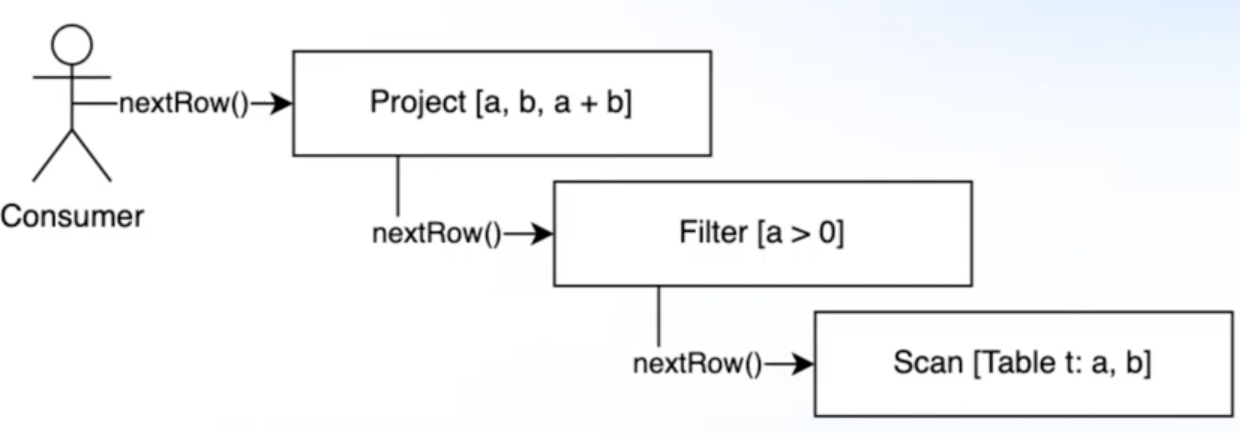
\includegraphics[width=\textwidth]{Pictures/Pull/Consumer pulls}
        \caption{Пример работы и подтягивании изменений}
    \end{figure}

    \begin{itemize}[label=+]
        \item Простота реализации
    \end{itemize}
    \begin{itemize}[label=-]
        \item Высокие накладные расходы на вызов \texttt{nextRow()}.
        Решение - возвращать список строк.
        \item Непредсказуемое исполнение.
        Не каждый вызов \texttt{nextRow} может вообще что-то вернуть (например \texttt{Filter}).
        \item Приостановка исполнения становится головной болью.
        \item Непонятно как распараллеливать выполнение оператора, что достаточно критично при обработке большого количества строк одним оператором.
    \end{itemize}

    \newpage

    \section*{Push based execution}

    Оператор не знает, кто его \texttt{input}, он только принимает на исполнение и в ответ отдаёт \texttt{output}

    \begin{lstlisting}[language=Java]
        interface Operator {
            void addInput(List<Row> rows);
            boolean needsInput();
            Optional<List<Row>> getOutput();
            Future<Void> isBlocked();
            boolean isFinished();
        }
    \end{lstlisting}

    \begin{itemize}
        \item \texttt{boolean needsInput()} --- некоторые операторы могут производить более, чем 1 выход в обмен на input, этот флаг позволит понять нужно ли оператору ещё данных или он всё ещё производит.
        \item \texttt{boolean isFinished()} --- приостановление оператора.
        \item \texttt{boolean isBlocked()} --- работа с сетью/диском/параллельно.
    \end{itemize}


\end{document}